\documentclass[times,11pt]{article}
%\usepackage[top=1cm, bottom=1cm, left=2.5cm, right=2.5cm]{geometry}

\usepackage{amsmath,amsfonts,amsthm}
\usepackage[pdftex]{graphicx}
\usepackage{float, caption, subcaption}
\usepackage{url}
\usepackage{natbib}

\numberwithin{equation}{section}		% Equationnumbering: section.eq#
\numberwithin{figure}{section}			% Figurenumbering: section.fig#
\numberwithin{table}{section}				% Tablenumbering: section.tab#

\graphicspath{ {./images/} }

%%% MACROS %%%

\newcommand{\ltwonorm}[1]{\left|\left|{#1}\right|\right|}
\newcommand{\xvec}{\mathbf{x}}
\newcommand{\HW}{\textsc{Hogwild!}}
\newcommand{\RR}{\mathbb{R}}
\newcommand{\blocks}{\mathcal{B}}
\newcommand{\neighs}[1]{\mathcal{N}\left({#1}\right)}
\newcommand{\Ocal}{\mathcal{O}}
%%%%%%%%%%%

\begin{document}

\title{Cache-Friendly Shuffles for Asynchronous Stochastic Optimization}
\author{Maximilian Lam, Horia Mania, and Maxim Rabinovich}

\maketitle
\section{Introduction}

In modern machine learning, many problems can be cast as instances of optimization, where the goal is to minimize some loss
function encoding the model's errors on training data. The ubiquity of such problems has led to substantial interest in making large-scale
optimization as efficient as possible, and a substantial portion of this work has focused on 
developing parallel asynchronous  algorithms that can under certain regimes
achieve near-ideal speedups in shared-memory systems.

% Introduce Hogwild.
So called {\it stochastic} optimization algorithms have found particular success in this regard. These algorithms, of which stochastic gradient descent (SGD) is the simplest example, operate
on problems whose loss functions decompose as a sum over datapoints:
\begin{align}
\label{eq:main-loss}
F\left(x\right) & = \sum_{i = 1}^{n} f_{i}\left(x\right) .
\end{align}
SGD proceeds by iteratively pulling out the loss function $f_{i}$ for a specific datapoint, updating the model $x$ based on that data point alone, and then moving on to the next one.
SGD and its close cousins have the advantage of being simply parallelizable. Indeed, the \HW{} algorithm~\cite{niu2011hogwild} simply spawns $p$ threads on single machine to perform single data point updates in parallel, updating the model stored in shared memory without any synchronization whatsoever. Perhaps surprisingly, this lock-free asynchronous approach works well for many problems, and since it avoids communication entirely, we might hope to achieve ideal speedups and thereby solve even the largest optimization problems facing machine learning practitioners.

% Theory.
% Explain systems issues at high level.
There have been numerous variants of this method proposed and under variants sets of assumptions theoretical analyses show that under different regimes one should expect speedups in practice~\cite{niu2011hogwild, lian2015asynchronous, reddi2015variance, de2015taming, liu2015asynchronous}. In \cite{mania2015perturbed}, the authors show under weak assumptions that as long as the number of processors are $\Ocal(n)$, where $n$ is the number of data points, \HW{} satisfies the same convergence rate as serial SGD. Therefore, one would hope that as long as the number of processors is not too large compared to the number of data points of the data set, \HW{} achieves nearly ideal speedup. 


Unfortunately, the simple story fails for a number of reasons, many of them systems-related. As the number of threads becomes large, the architecture of the machine
imposes limitations and tradeoffs that must be taken into account. For instance, many machines with sufficiently many cores to support parallelism beyond approximately $16$
threads organize their cores in a non-uniform memory access (NUMA) architecture, meaning that implementations of Hogwild must either cope with potentially long cross-NUMA node
accesses to the memory storing the model or alter the algorithm so that cores on a given node usually only access memory on that node. When moving to multiple machines,
alterations to the algorithm become not only desirable but absolutely necessary.

% Discuss related work (e.g. DimmWitted, Downpour) on multi-node/multi-machine setting
A great deal of work has gone into understanding the statistical and computational properties of multi-node and multi-machine versions of the algorithm~\cite{zhang2014dimmwitted, dean2012large}. The recent DimmWitted system
explored the design space of Hogwild-type algorithms in significant detail, tuning several knobs like: how much of the data each thread used; whether independent copies of the model were stored by each thread,
or only on each NUMA node, or whether only a single global version of the model was maintained at all times; and how often threads received updated versions of other threads' models in the case of model replication. They
found substantial differences in performance across these settings, and identified important computational-statistical tradeoffs to guide further work. In prior work~\cite{dean2012large}, the authors had undertaken a similar study in the rather different multi-machine setting.

% Pivot to single-node case (ref Jellyfish, Buckwild).
Comparatively little attention has been paid to the simpler setting of a single node, despite the fact that failing to take the memory access pattern into account can limit the speedup from parallelization
both on the individual node in isolation and in the context of larger multi-node or multi-machine systems. A notable exception to this general trend is the Jellyfish system for large-scale matrix factorization, which employs a 
blocking scheme to ensure that no two threads access the same parameters in any given epoch---a design choice that also ensures a high degree of cache locality within each thread's memory accesses since each thread's 
assigned block depends only on a fraction of the total model parameters~\cite{recht2013parallel}. And more recently, further support for the idea that memory access optimizations can greatly increase the efficiency of optimization algorithms
has come from work showing that low-precision arithmetic variants of the Hogwild algorithm can achieve substantially better speedups than their high-precision predecessors~\cite{de2015taming}.

% Introduce our approach
In this report, we investigate a general-purpose methodology for optimizing the memory access efficiency of Hogwild-style algorithms. Building on the Jellyfish results, we propose to group datapoints into blocks that each access only a 
limited subset of the parameters and to use these blocks to constrain the order in which threads access datapoints. We hypothesize that, if the blocking is done well, this strategy will have the effect of increasing cache hits on model parameters within a single thread.
Further, if different threads are further required to iterate through the blocks in different orders, we expect it to have the additional beneficial effect of reducing conflicting model accesses across threads, thereby also decreasing performance losses due to cache coherence effects.

The remainder of this report elaborates on our approach and provides evidence for these hypotheses. In Section~\ref{sec:alg-spec}, we explain the details of our proposed algorithm and introduce the bipartite datapoint-parameter dependence graph that underlies it. In Section~\ref{sec:memory-model}, we provide a simple 
two-level memory model analysis of the \HW~ algorithm and frame the problem of optimally blocking datapoints as a graph partitioning problem in the dependence graph. In Section~\ref{sec:ls}, we investigate how the structure of the datapoint-parameter graph affects the potential gains from 
effective blocking. In Section~\ref{sec:w2v}, we go on to show that a particular blocking strategy based on iterated min-cut can achieve substantial gains, both in runtime and speedup, on a real machine learning problem, namely the learning task for the popular Word2Vec model for word embeddings~\cite{arora2015rand}. Finally, in 
Section~\ref{sec:conc}, we reflect on our results and propose several avenues for further work.

\section{Block-Constrained Shuffling}\label{sec:alg-spec}

Our approach to making \HW~ memory access efficient hinges on constraining the order in which the algorithm processes data points. Typically, each thread
in the algorithm processes the data points in a randomly selected thread-specific ordering, meaning that the data
point processed by a thread at some iteration $j$ need not share any parameters with the data point processed at iteration $j - 1$ or $j + 1$. In practice, the 
common approach involves shuffling the data points and then iterating over them in order. In theory, for ease of analysis, it is common to assume that at each iteration
a data point is sampled uniformly at random with replacement. 
However, these approaches have little cache locality. We aim to remedy this defect.

Specifically, we aim to group the datapoints into blocks that mostly depend on the same parameters, and such that each block depends only a comparatively small number of 
distinct parameters. Given this blocking, we constrain the order in which threads process datapoints to be consistent with the blocking. Here consistency means that, as the thread iterates through
the data, once it has processed a data point from some block, it will not process any more data points outside that block until it has finished with the entire block.

We can make the algorithm specification more precise as follows. Let the blocks of data points be given by $\blocks = \lbrace B_{1}, \dots, B_{K} \rbrace$, where each $B_{k} = \lbrace i_{k1}, \dots, i_{km_{k}}\rbrace$ is a set of data point indices. Then we assume that the sequential ordering
$I_{p} = \left(i_{p1}, \dots, i_{pn}\right)$ according to which thread $p$ processes data points has the form $\left(I_{pa_{1}}, \dots, I_{pa_{K}}\right)$, where each $I_{pa_{k}}$ is an ordering of the indices in $B_{k}$. 

We point out, anticipating the analysis in Section~\ref{sec:memory-model}, that the problem of choosing good blocks of data points  bears a strong resemblance to the graph partitioning problem that arises in sparse matrix-vector multiply. The difference is that the dependence graph for our problem
links datapoints to parameters and therefore has a bipartite structure. The blocking problem is then simply a graph partitioning problem on one side of this graph. 

To highlight this point, we index the individual functions $f_{e_i}$ in~\eqref{eq:main-loss} by subsets $e_i \in \lbrace 1, 2, \ldots, d \rbrace$, where $d$ is the dimension of $\xvec$, instead of plain numerical indices $i$. Then, we 
assume that each function $f_{e_i}(\xvec)$ depends only on coordinates of $\xvec$ indexed by the subset $e_i$. In particular, $\nabla f_{e_i}(\xvec)_v = 0$ for all $v\not \in e_i$. Then, we construct a bipartite graph by having the functions $f_{e_i}$ on one side and the coordinates of $\xvec$ on the other side. We connect a function $f_{e_i}$ to a coordinate $v$ if $v\in e_i$.   

\section{A Simplified Memory Model Analysis}\label{sec:memory-model}

Simplified memory models can provide useful guidance when optimizing algorithm performance, as the case of matrix-matrix multiply illustrates. In this section, we use a two-level memory model to estimate the computational intensity of the algorithm
in terms of the blocking structure and use the resulting estimate to formalize the problem of finding an optimally memory access efficient blocking as a graph partitioning problem in the datapoint-parameter graph described in Section~\ref{sec:alg-spec}.

Concretely, assume the memory hierarchy has two levels, fast and slow, where fast memory contains sufficient storage for $M$ model parameters and has zero access cost. We assume further that reads and writes have equal cost and that the computational effort required to obtain the model update based on datapoint $i$ is proportional to the cardinality $|e_{i}|$, say equal to $c|e_{i}|$ for some absolute constant $c > 0$. 

Note that under this framework, a model update based on datapoint $i$ requires $|e_{i}|$ parameter reads to compute the update, $c|e_{i}|$ steps of computation (e.g. flops) to compute the update, and $|e_{i}|$ parameter writes to actually perform the update. 

Now let the order in which a thread performs updates based on data points be $I = \lbrace i_{1}, \dots, i_{n}\rbrace$. To process data point $i_{j}$, the
algorithm needs to read in some number $r_{j}\left(I\right)$ of model parameters to perform the update; the remaining $|e_{i_j}| - r_{j}\left(I\right)$ are
already in fast memory and therefore cost nothing to access. The total number of reads is therefore given by $\sum_{i = 1}^{n} |e_{i}| - \sum_{j = 1}^{n} r_{j}\left(I\right)$, while the total number of writes is given by $\sum_{i} |e_i|$. The computational intensity can therefore be written as
\begin{align}
q\left(I\right) & = \frac{c\sum_{i = 1}^{n} |e_{i}|}{\sum_{i = 1}^{n} |e_{i}| + \sum_{j = 1}^{n} r_{j}\left(I\right)} . 
\end{align}
The problem of maximizing $q$ is therefore equivalent to the problem of minimizing the sum
\begin{align}
r\left(I\right) & = \sum_{j = 1}^{n} r_{j}\left(I\right) . 
\end{align}

In the context of the blocking algorithm, we can bound $r\left(I\right)$ as follows. Let the blocking structure be given by $\blocks = \lbrace B_{1}, \dots, B_{K} \rbrace$. Let $m_{k}$ be the number of distinct parameters touched by block $k$, or, more formally, $m_{k} = \left|\cup_{i \in B_{k}} e_{i}\right|$, which is also
equal to the number of neighbors of $B_{k}$, $\neighs{B_{k}}$, in the datapoint-parameter dependence graph. Provided each $m_{k}$ is bounded by the fast memory size $M$, we have
\begin{align}
r\left(I\right) & \leq \sum_{k = 1}^{K} m_{k} . 
\end{align}
Writing $m_{k} = \left|\neighs{B_{k}}\right|$, we thus find that the graph partitioning problem we face can be formulated as
\begin{align}\label{eq:comb-opt}
\min \sum_{k = 1}^{K} \left|\neighs{B_{k}}\right| ~~ \text{subject to}~~ \left|\neighs{B_{k}}\right| \leq M,~ 1 \leq k \leq K .
\end{align}

As this problem bears a strong resemblance to the NP-hard set cover problem~\cite{arora2009computational}, we do not attempt to solve it exactly. Instead, we investigate three heuristics for solving it:
\begin{enumerate}
\item
{\bf Truncated breadth-first search.} In this approach, we do not fix the number of blocks in advance. Instead, we iterate through the data points and whenever we encounter one that has not yet been assigned a block, we start a breadth-first search for datapoints to put in a new block including the data point initiating the 
search. Whenever the search encounters a data point that has not yet been assigned to a block, it adds it to the new block and enqueues all of its neighbors that have not themselves been assigned to a block. The search halts either when the queue is empty, or when the number of data points assigned to he new block
exceeds a client-specified threshold.

\item
{\bf Greedy streaming.} In this approach, we fix the number of blocks before the algorithm starts. Then, we iterate through the data points and at each step, add the next data point to the block $B_{k}$ that makes the objective in~\eqref{eq:comb-opt} as small as possible.
\item
{\bf Iterated min-cut.} In this approach, we again fix the number of blocks in advance, specifically setting $K = 2^{\kappa}$, where $\kappa \geq 0$ is a depth parameter. We then perform $\kappa$ recursive min-cuts and keep the bottom level of the resulting hierarchical blocking.
\end{enumerate}

\section{Least Squares}\label{sec:ls}

We have chosen least squares as a first application for testing the gains brought by cache friendly shuffles.
More precisely, we  implemented the \HW{} method for optimizing the least squares objective 
\begin{equation}
\label{eq:LS}
F(\xvec) = \sum_{i = 1}^n \ltwonorm{\langle a_i, \xvec \rangle - b_i}^2,
\end{equation}
where $a_i, \xvec \in \RR^d$ and $b_i\in \RR$. 
At each iteration the algorithm chooses a data-point $(a_i, b_i)$, it reads the coordinates of the model $\xvec$ that belong to the support of the vector $a_i$, computes the gradient $2(\langle a_i, \xvec\rangle - b_i)a_i$, and updates the model $\xvec$ accordingly in shared memory.

The benefits of working with this problem are twofold. Firstly, it is easy to see the correspondence between the data points $(a_i, b_i)$ and the bipartite graph described in Section~\ref{sec:alg-spec}. Each data point $(a_i,b_i)$ is connected to the coordinates of $\xvec$ that belong to the support of $a_i$. Therefore, we can easily generate synthetic data with different structures of the bipartite graph and test what properties of the bipartite graph impact performance. Secondly, the analysis of least squares yields insights into any optimization problem of the form 

\begin{equation}
F(\xvec) = \sum_{i = 1}^n \ell (\langle a_i, \xvec\rangle, b_i),
\end{equation}
where $\ell \colon \RR \times \RR \rightarrow \RR$ is some loss function. For example, the objective of a linear SVM takes this form. 


\subsection{Graph Structures Considered}

All the data sets we generated have $n = 3\cdot 10^6$ data points and $d = 10^4$ parameters. The non-zero entries of the data-points $(a_i, b_i)$ have been sampled uniformly from the interval $(-1,1)$.  We made these choices because on datasets of this size the standard \HW{} method achieves good speedup for up to $12$ threads. Therefore, on such data, we can observe what benefits our method brings in a setting where \HW{} performs well. 

\subsubsection*{Uniform}

To generate a datapoint $(a_i, b_i)$ under this model we sample uniformly at random and without-replacement a set of $k$ parameters (in our experiments we chose $k = 20$) out of the total $10^4$ parameters of $\xvec$ and connect the datat point $i$ to these parameters.  The corresponding coordinates of $a_i$ are sampled uniformly at random from $(-1,1)$ and the coordinates that do not have an edge connected to the data point are set to zero. The real value $b_i$ is uniformly sampled from $(-1,1)$. 

\subsubsection*{Preferential-Attachment}

A dataset under this model is generated sequentially. Firstly we connect the data point $(a_1, b_1)$ to a set of $k$ parameters chosen uniformly at random without replacement. Then, for each new data point $(a_i, b_i)$ we connect it to a $k$ parameters chosen without replacement with a probability proportional to their current degree in the bipartite graph (i.e. the number of datapoints that depend on them so far). Given the bipartite graph the coordinates of $(a_i, b_i)$ are either set to zero or sampled uniformly at random from $(-1,1)$. The datapoints are shuffled at the end.


\subsubsection*{Stochastic Block Model}

Under this model we group the parameters into disjoint sets of $k$-parameters. Denote by $b$ the number of groups of parameters obtained. Then, for each group of parameters choose without replacement $\lfloor \frac{n}{b}\rfloor$ data points and connect each of them to all of the parameters in the group. Finally, connect each data point to $k'$-parameters chosen uniformly from the blocks that do not correspond to that data point. The number $k'$ is called the \emph{cross-degree}. Under this model there is an implicit partition of the bipartite graph that optimizes the objective described in Section~\ref{sec:memory-model}, this partition is given by the groups of $\lfloor \frac{n}{b}\rfloor$ used to generate the graph. In our experiments we use this true partitioning of the graph to find the best possible gains that our method could yield assuming it finds the optimal partitioning.
   
\subsection{Experimental results}

We implemented the \HW{} algorithm for optimizing objective \eqref{eq:LS} in C++ and ran the experiments on the Edison compute nodes which feature two twelve core 2.4 GHz processors. 
Nonetheless, to avoid undesirable effects due to non-uniform memory accesses, we used up to twelve threads and pinned them to individual cores of one NUMA node. 

In Figures~\ref{fig:unif} and~\ref{fig:pref} we compare the standard \HW{} method with our version of the algorithm on two problems having the uniform structure and preferential attachment structure respectively. To compute the data point blocks we used the greedy-streaming algorithm described in Section~\ref{sec:memory-model}. We observe no gains from using our method for these graph structures. These results are unsurprising since graphs generated by uniform and preferential-attachment models have no true underlying block structure. Therefore, there is no way of partitioning the graphs so that we obtain gains in the sense of Section~\ref{sec:memory-model}. Nonetheless, it is reassuring to see that our method does not perform worse than the standard \HW{} algorithm. 

\begin{figure}[h!]
\centering
    \begin{subfigure}[b]{0.49\columnwidth}
	\centerline{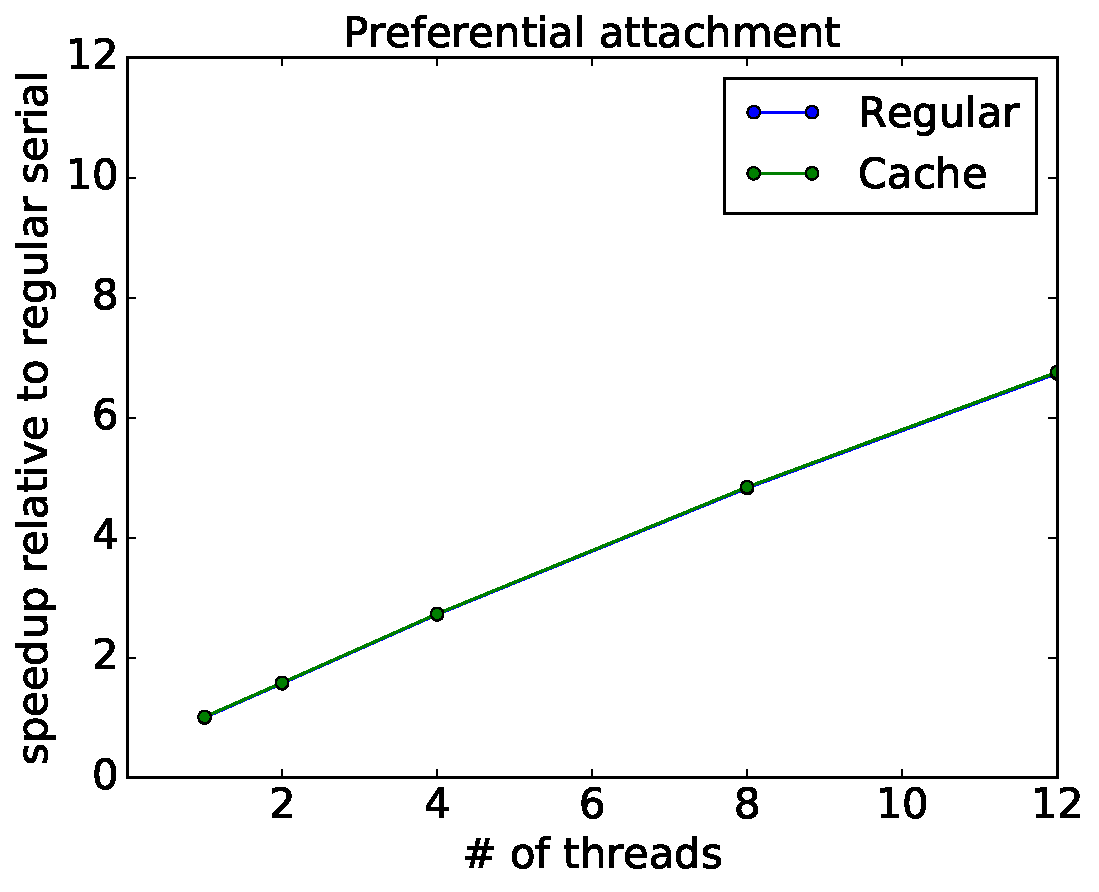
\includegraphics[width = 0.85\columnwidth, trim={0 0.1cm  0 0}, clip]{LS_speedup_prefattach.pdf}}
      \caption{\scriptsize Uniform Bipartite Graph}
      \label{fig:unif}
    \end{subfigure}
   \begin{subfigure}[b]{0.49\columnwidth}
      	\centerline{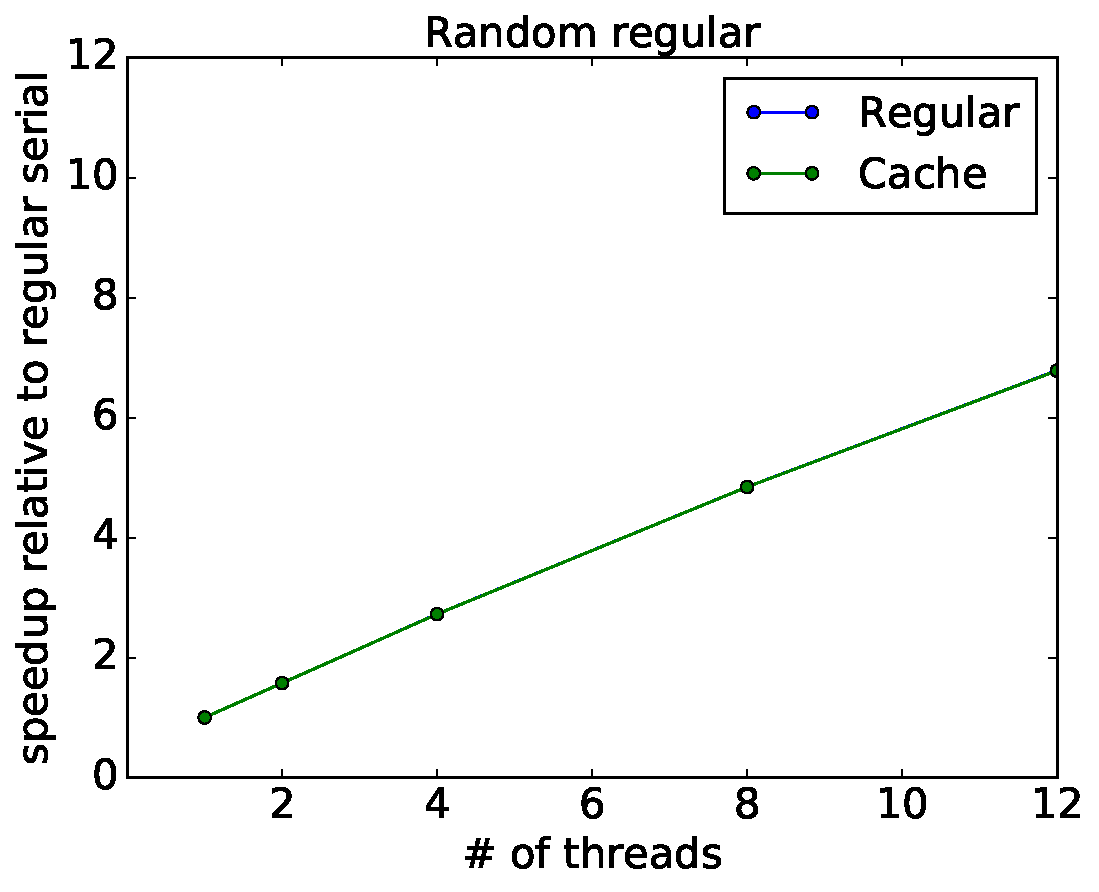
\includegraphics[width = 0.85\columnwidth, trim={0 0.1cm  0 0}, clip]{LS_speedup_regular.pdf}}
      \caption{\scriptsize Preferential-Attachment Bipartite Graph}
      \label{fig:pref}
    \end{subfigure}
  \caption{Plotting speedup as a function of the number of threads for problems generated according to the Uniform and Preferential-Attachment models. The problems have $3$ million datapoints and $10000$ parameters. Each datapoint depends on $20$ parameters.}
  \label{fig:unif-pref}
\end{figure}
 
Figures~\ref{fig:pcross0} \ref{fig:pcross0.1}, \ref{fig:pcross0.5}, \ref{fig:pcross1} show the same comparison for the stochastic block model for different values of the cross-degree. To measure the ideal gains we could hope to obtain from the 
cache-friendly shuffles we use the true blocks to generated the shuffles. We have noticed similar gains by using the greedy streaming algorithm for small values of the cross degree. 

\begin{figure}[h!]
\centering
    \begin{subfigure}[b]{0.49\columnwidth}
	\centerline{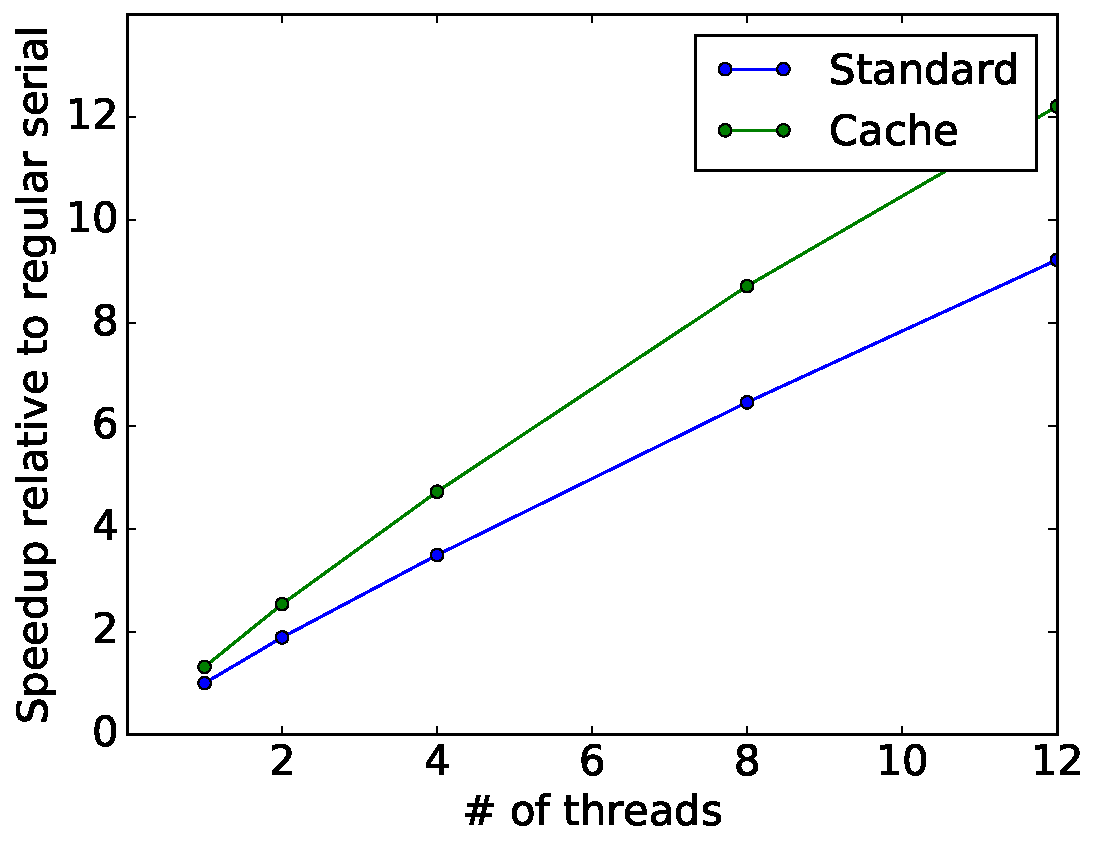
\includegraphics[width = 0.85\columnwidth, trim={0 0.1cm  0 0}, clip]{report_LS_speedup_blockmodel_pcross=0.pdf}}
      \caption{\scriptsize Cross degree 0}
      \label{fig:pcross0}
    \end{subfigure}
   \begin{subfigure}[b]{0.49\columnwidth}
      	\centerline{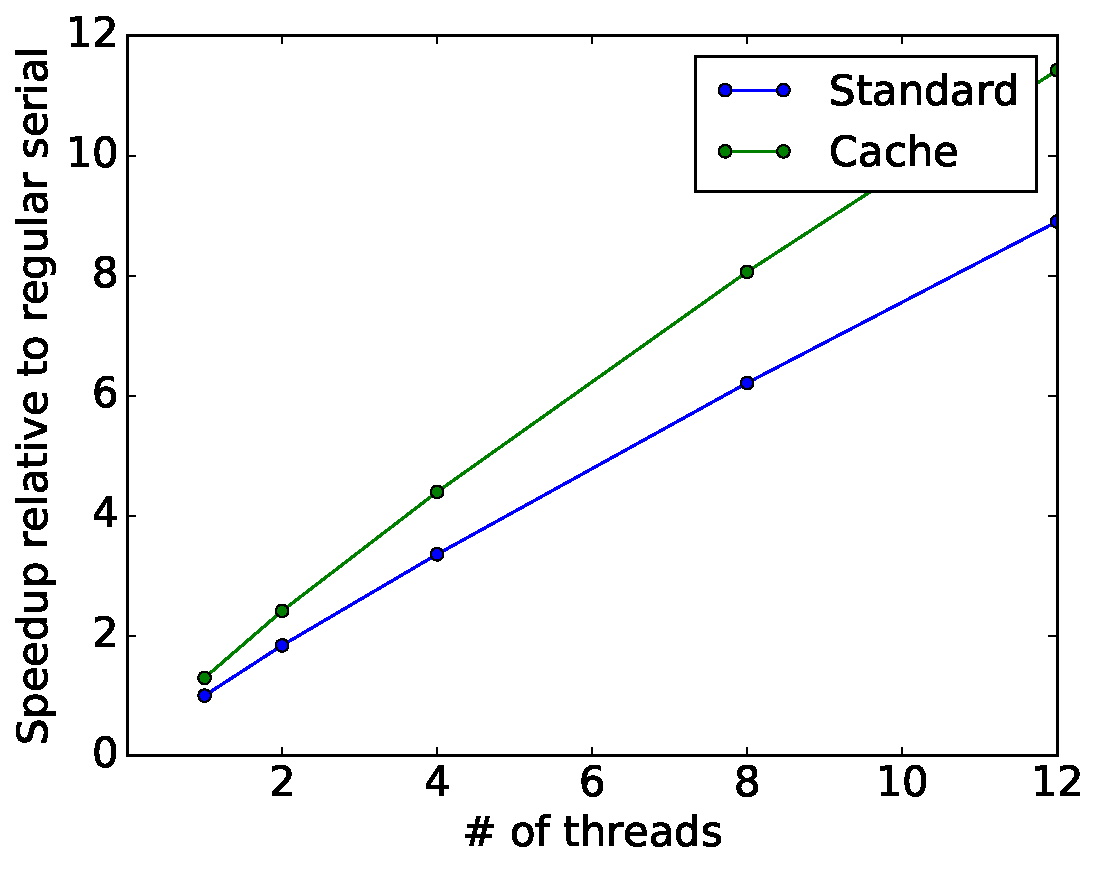
\includegraphics[width = 0.85\columnwidth, trim={0 0.1cm  0 0}, clip]{report_LS_speedup_blockmodel_pcross=01.pdf}}
      \caption{\scriptsize Cross degree 2}
      \label{fig:pcross0.1}
    \end{subfigure}
 \begin{subfigure}[b]{0.49\columnwidth}
	\centerline{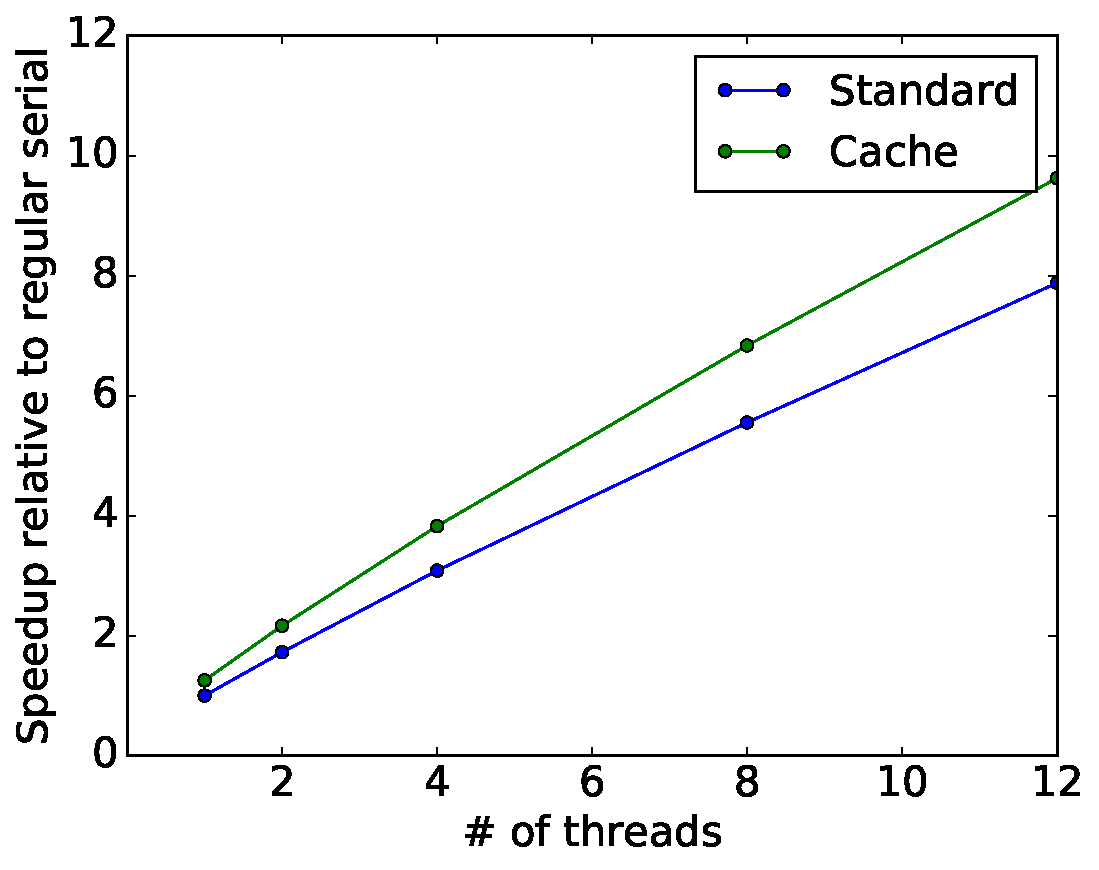
\includegraphics[width = 0.85\columnwidth, trim={0 0.1cm  0 0}, clip]{report_LS_speedup_blockmodel_pcross=05.pdf}}
      \caption{\scriptsize Cross degree 10}
      \label{fig:pcross0.5}
    \end{subfigure}
   \begin{subfigure}[b]{0.49\columnwidth}
      	\centerline{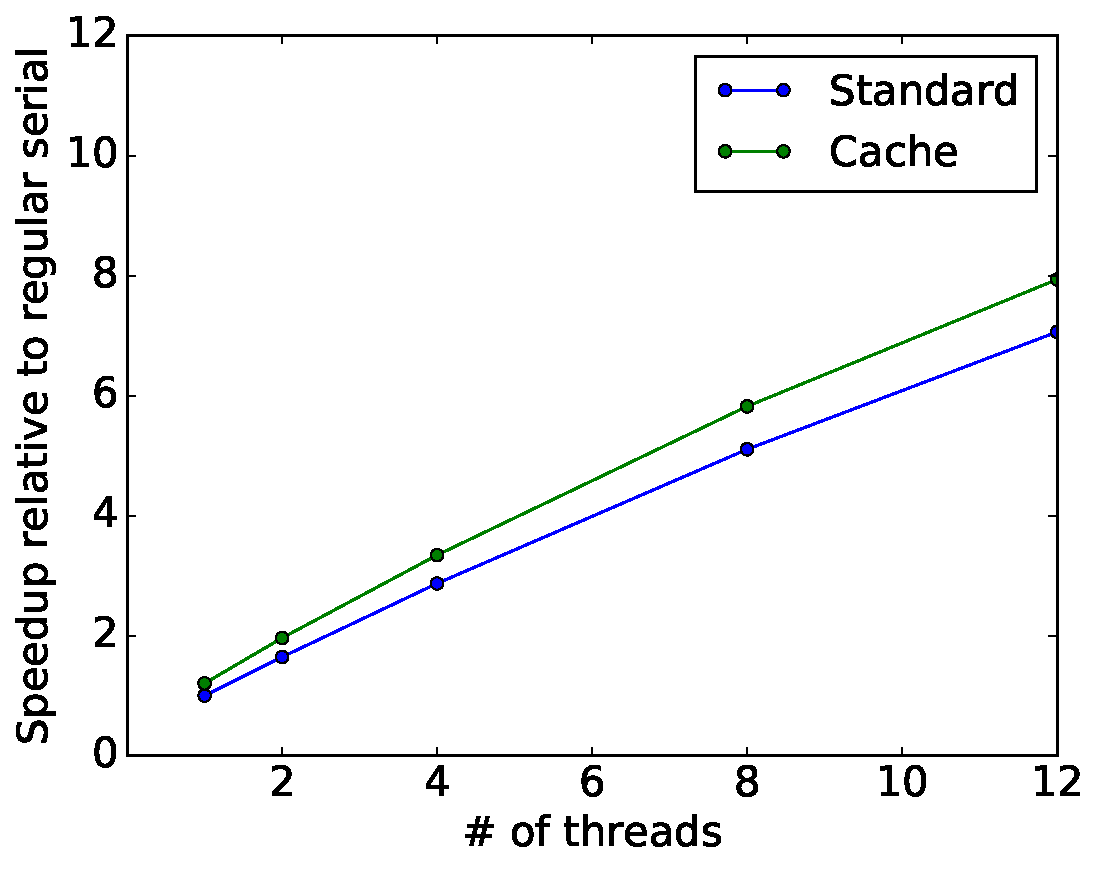
\includegraphics[width = 0.85\columnwidth, trim={0 0.1cm  0 0}, clip]{report_LS_speedup_blockmodel_pcross=1.pdf}}
      \caption{\scriptsize Cross degree 20}
      \label{fig:pcross1}
    \end{subfigure}
  \caption{Plotting speedup as a function of the number of threads for problems generated according to the stochastic block model. The problems have $3$ million datapoints and $10000$ parameters. Each datapoint depends on $20$ plus the cross-degree parameters.}
  \label{fig:unif-pref}
\end{figure}

In these experiments we observe an additive gain from using the cache-friendly shuffles, for the different values of the cross-degree. Our method performs better by approximately $10$ seconds when using $1$ thread regardless of the cross degree, and the gain gets halved each time we double the number of threads used. This behavior occurs because the number of times a parameter is accessed in the L1-cache remains constant with increasing values of the crossing-degree (for small enough crossing-degree). 


To show that the gains are additive in Figure~\ref{fig:crossratio} we plot the ratio of the gain and the running time of standard serial \HW{} as a function of cross degree.
\begin{figure}[h!]
\centering
    \begin{subfigure}[b]{0.49\columnwidth}
	\centerline{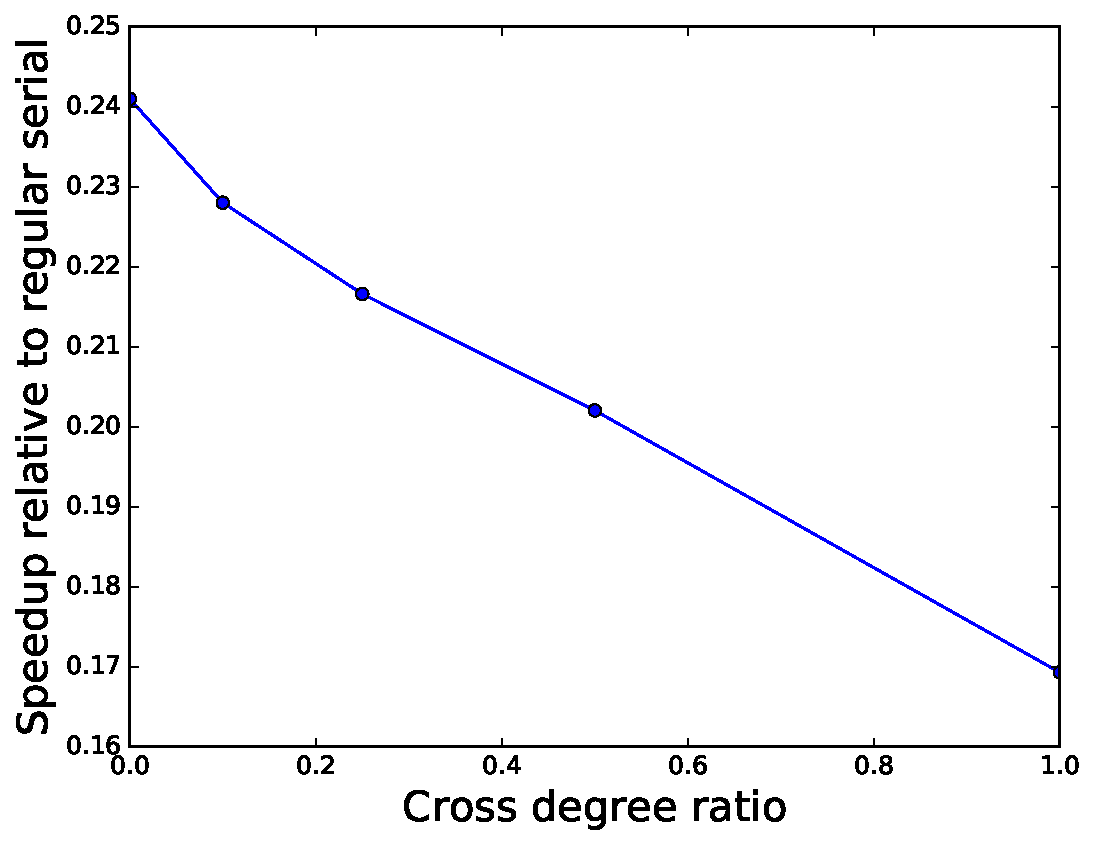
\includegraphics[width = 0.85\columnwidth, trim={0 0.1cm  0 0}, clip]{report_serial_cache_gains.pdf}}
      \caption{\scriptsize }
      \label{fig:crossratio}
    \end{subfigure}
  \caption{The ratio of the gain and the running time of standard serial \HW{} as a function of cross degree.}
\end{figure}

\section{Word Embeddings}\label{sec:w2v}

\subsection{Problem statement}
In the word embeddings problem, given context counts $X_{w,w'}$ we want to find word vectors
$v_{w} \in \mathbb{R}^{k}$ that minimizes the loss:
\begin{align*}
\min_{v,C}\sum_{w,w'}X_{w,w'} \left(\log(X_{w,w'}) - \ltwonorm{v_w+v_{w'}}^2 - C\right)^2
\end{align*}

\subsection{Experimental evaluation}
\subsubsection{Methodology}

We ran our experiments on the Edison compute nodes which feature two
twelve core 2.4 GHz processors. However, we used only up to twelve
cores/threads to avoid effects of NUMA. Word vectors were length 100
double arrays.
\\\\
We used the first $10^9$ bytes of English Wikipedia from
http://mattmahoney.net/dc/textdata as corpus data. After running the text
preprocessing script supplied by the link, we computed co-occurrence
counts of pairs of distinct words to create the parameter dependence graph.
This graph was then fed into gpmetis, computing a min-k-cut partitioning to
create a cache-friendly ordering of the datapoints. k was set such that each
block of k datapoints would reference just enough word vectors to fit into the
L1-cache.
\\\\
Hogwild was then run on the permuted co-occurrence graph generated by gpmetis,
maintaining the same ordering throughout execution. Although we experimented with
both data sharding and no-data sharding, only results from data sharding are presented.
To test hogwild without a cache-friendly shuffle, we randomly shuffled the datapoints before execution.
\\\\
We also ran the experiments on subsets of the corpus, repeating the
procedure on the first $\%10$, $\%25$, $\%50$ and $\%75$ of the corpus data.
In the full corpus data, there were $~200,000$ word vectors, and $~30,000,000$
datapoints.

\subsubsection{Results}
\noindent We achieve between $\%40-\%50$ speedup over regular hogwild (non-cache-friendly hogwild),
measuring runtime to a fixed number of epochs.
\begin{figure}[H]
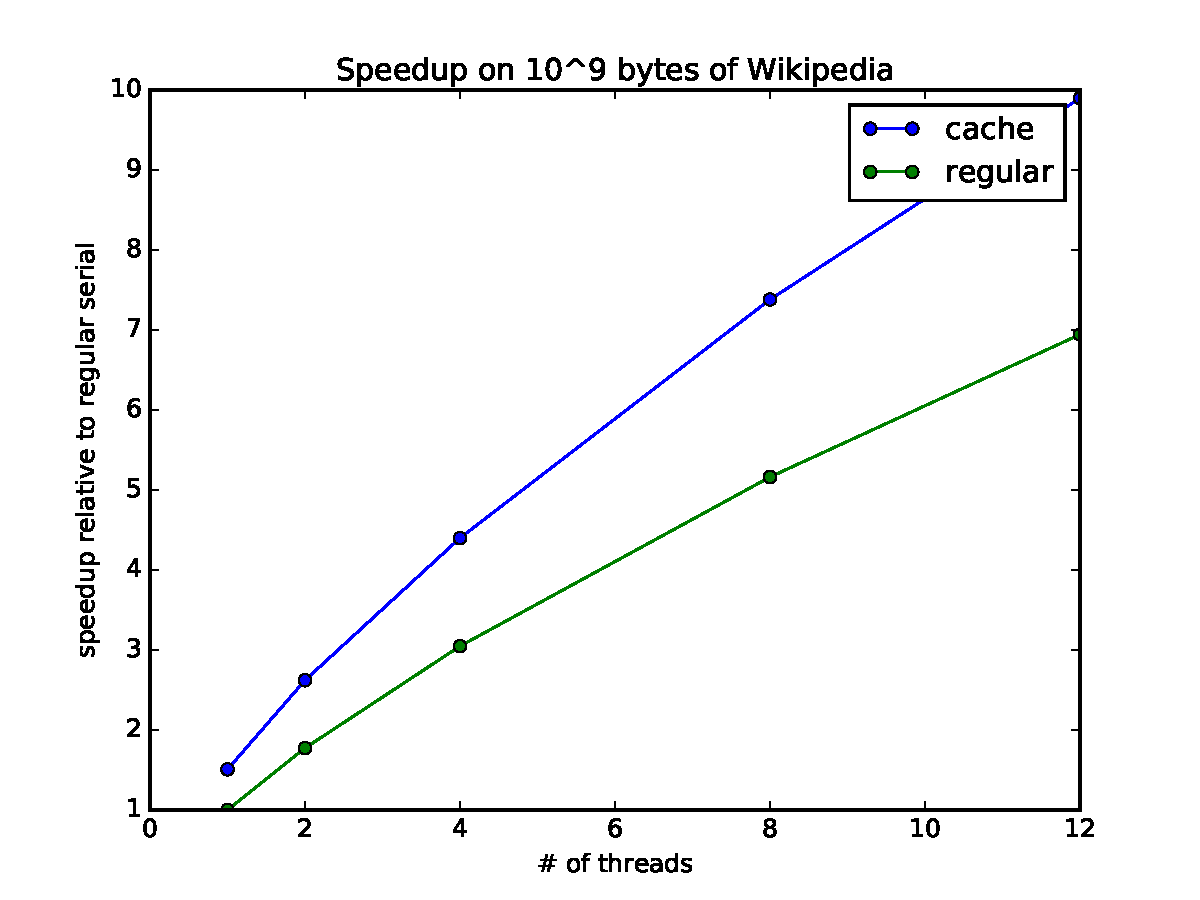
\includegraphics[width=11cm,height=11cm,keepaspectratio]{w2v_speedup_plot.pdf}
\end{figure}
\noindent Furthermore, the speedup is maintained on different subsets and sizes of the data.
\begin{figure}[H]
\begin{center}
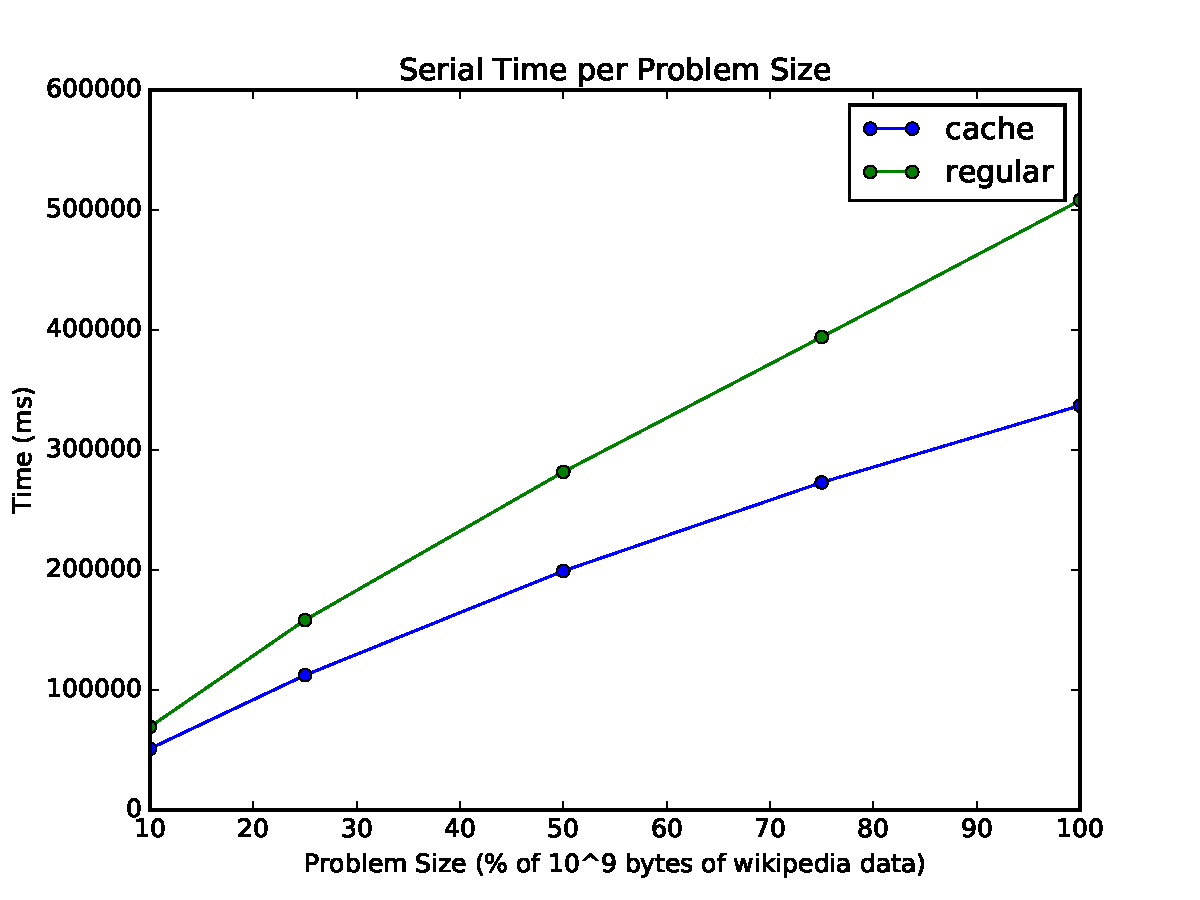
\includegraphics[width=11cm,height=11cm,keepaspectratio]{w2v_problem_size_time_plot.pdf}
\end{center}
\end{figure}
\noindent Additionally, convergence of loss is not adversely affected.
\begin{figure}[H]
\begin{center}
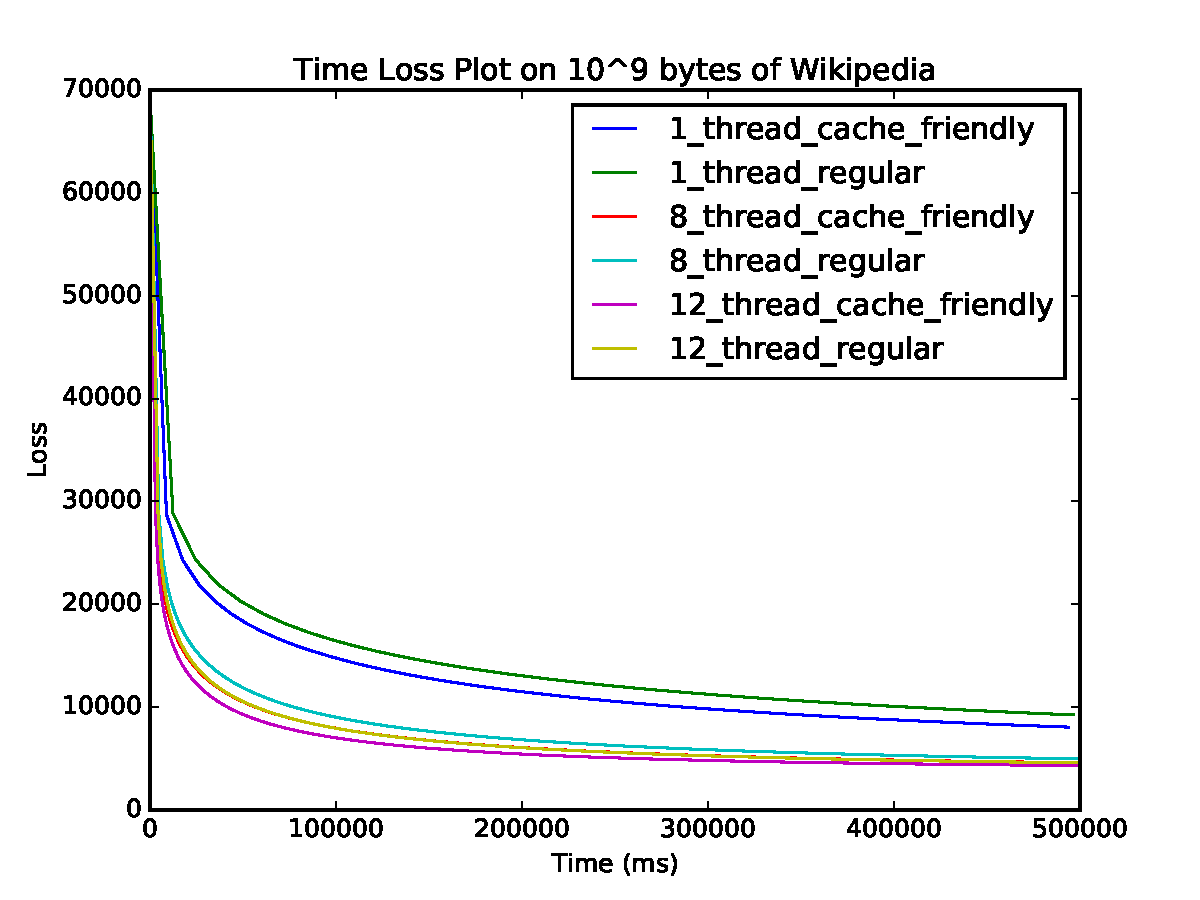
\includegraphics[width=11cm,height=11cm,keepaspectratio]{w2v_time_loss_plot.pdf}
\end{center}
\end{figure}

\subsection{Discussion}

A $\%40-\%50$ runtime gain over regular hogwild is a result of keeping
at least one length 100 double array in the L1-cache between
stochastic gradient calls. In a non-cache-friendly permutation, each
of the two vectors visited by a datapoint is typically not in the
cache, incurring two vectors worth of cache misses per
datapoint. After running min-k-cut on the parameter dependence graph,
we found that each block of k datapoints references around k distinct
vectors. Thus, in a cache-friendly permutation, one of the vectors
referenced by a datapoint is already in the L1-cache from the previous
stochastic gradient call. So a cache-friendly permutation incurs only
one vectors worth of cache misses per datapoint, naturally leading to
a $\%40-\%50$ reduction in runtime.

\section{Conclusion and future directions}\label{sec:conc}
%By ordering datapoints so that model parameters are accessed in a cache friendly manner, we achieve substantial runtime reductions.

% Conclusion for LS

% Conclusion for W2V
%For word embeddings, we achieve a $\%40-\%50$ runtime gain over regular hogwild by ordering the datapoints via min-k-cut.

% Overall Conclusion
%From these results we believe that using a cache friendly shuffling of datapoints is a promising approach to reducing the runtime of stochastic optimization methods.

% Future directions
%The runtime gains achieved by using a cache-friendly shuffle is highly
%contingent on the structure of the parameter depedence graph and on
%the method used to permute the datapoints. Thus, one possible
%direction to explore is the behavior of cache-friendly shuffles on
%different graph structures and problem types. We may find that graph
%properties such as sparsity, etc, have a nontrivial effect on the
%efficacy of cache-friendly shuffles.
%\\\\
%Different shuffling methods may be another topic of exploration, particularly
%the tradeoff between computational efficiency and shuffle
%quality. Investigating different greedy methods and heuristics for
%greedy shuffles may reveal computationally efficient methods for
%generating a quality cache shuffe. On the other hand, it may also be
%interesting to see how effective optimal shuffles are, perhaps by
%generating them through some sort of integer linear programming
%routine.
%\\\\
%Finally, a shuffling that takes advantage of all levels of cache may yield further runtime gains.
%Thus, a cache-oblivious shuffling method may be yet another area to explore.

In this report, we have demonstrated the potential for substantial performance gains from cache awareness in asynchronous optimization algorithms. We proposed
to achieve cache awareness by constraining the order in which the algorithms process datapoints. Based on a simple two-level memory model, we argued that the constraint
should come from a blocking obtained by solving a certain graph partitioning problem in the bipartite datapoint-parameter graph. We then showed that on synthetic sparse least-squares
datasets, good performance gains could be achieved if the true underlying blocking was known. Finally, we showed that an iterated min-cut heuristic for solving the graph partitioning problem
produced blockings that gave significant performance gains on the popular Word2Vec benchmark task.

Our work raises a variety of further questions. On one hand, we have questions about the fundamental limitations of cache-awareness for improving the efficiency of these algorithms.
How much of the deviation from ideality can be explained by cache non-locality and how much comes from other sources? And even when cache non-locality is the primary inefficiency,
it is far from clear what degree of locality we can expect to achieve; some graphs simply exhibit a high degree of interconnection that makes blocking impossible. It would therefore be of interest
to investigate in greater depth the preferential attachment and uniformly random graph structures we briefly analyzed in Section~\ref{sec:ls} in order to see what sorts of gains might be achieved for
those topologies.

On the other hand, we have algorithmic questions essential to developing practical implementations of our approach. Although iterated min-cut worked well for Word2Vec, it imposed a heavy computational burden, and we would like
to find more efficient ways to achieve the same result. The other heuristics we tried, on the other hand, were either inefficient or ineffective or both. It would therefore be of significant research interest to 
investigate the use of alternate large-scale graph partitioning algorithms for these problems and see if they can do well---for this, both classical spectral approaches and more modern methods based on submodular optimization
might come in useful.

Finally, we have only touched on a couple of the myriad tasks machine learning practitioners use asynchronous stochastic optimization algorithms to solve. To fully understand the reach of our method, we hope in future work to 
benchmark it on other problems that exhibit different graph structures and thus perhaps different computational properties.

\bibliographystyle{unsrt}
\bibliography{report}


\end{document}

%%% Local Variables:
%%% mode: latex
%%% TeX-master: t
%%% End:
